\documentclass{article}

\usepackage{tabularx}
\usepackage[table]{xcolor}
\usepackage{hyperref}
\usepackage{cleveref}
\usepackage{tikz}
\usetikzlibrary{positioning, calc, shapes, arrows, fit}
\usepackage{circuitikz}
\usepackage{subcaption}
\usepackage[colorinlistoftodos]{todonotes}
\linespread{0.9}
\hypersetup{
    colorlinks = true,
    linkbordercolor = {black}
}
\begin{document}
\title{Lab 1 -- Measuring ``Parasitics'' of Passive Components with a VNA}
\author{
    Yifan Zhu\\
    Lab Partner: John Kustin
}
\maketitle

\begin{abstract}
    S-Parameters of passive components are measured using a Vector Network Analyzer (VNA), and more realistic circuit models containing parasitics are proposed.
    The proposed circuit models are simulated in LTSPice, and compared against the experimentally obtained results.
\end{abstract}

\section{Introduction}
Real life passive components are far from ideal.
All capacitors, inductors, and resistors have some parasitic capacitance, inductance, and resistance.
But how can we measure these parasitics?
How can we build good electric models of these real-world componenets?
To this end, we use Vector Network Analyzers (VNA) to measure the frequency response of these passive components, use our understanding of circuit elements to conjecture about good circuit models, and use LTSpice to verify that the circuit models match what we observe.

\section{Experimental Setup}
The passive componenets of interest are all surface mount components on the \emph{RF Demo Kit NWDZ Rev-01-10} (\Cref{fig:test_loads}), and
we use the NanoVNA (\Cref{fig:nanovna}) to perform the measurements.
\begin{figure}[h]
    \centering
    \begin{subfigure}{.5\linewidth}
        \centering
        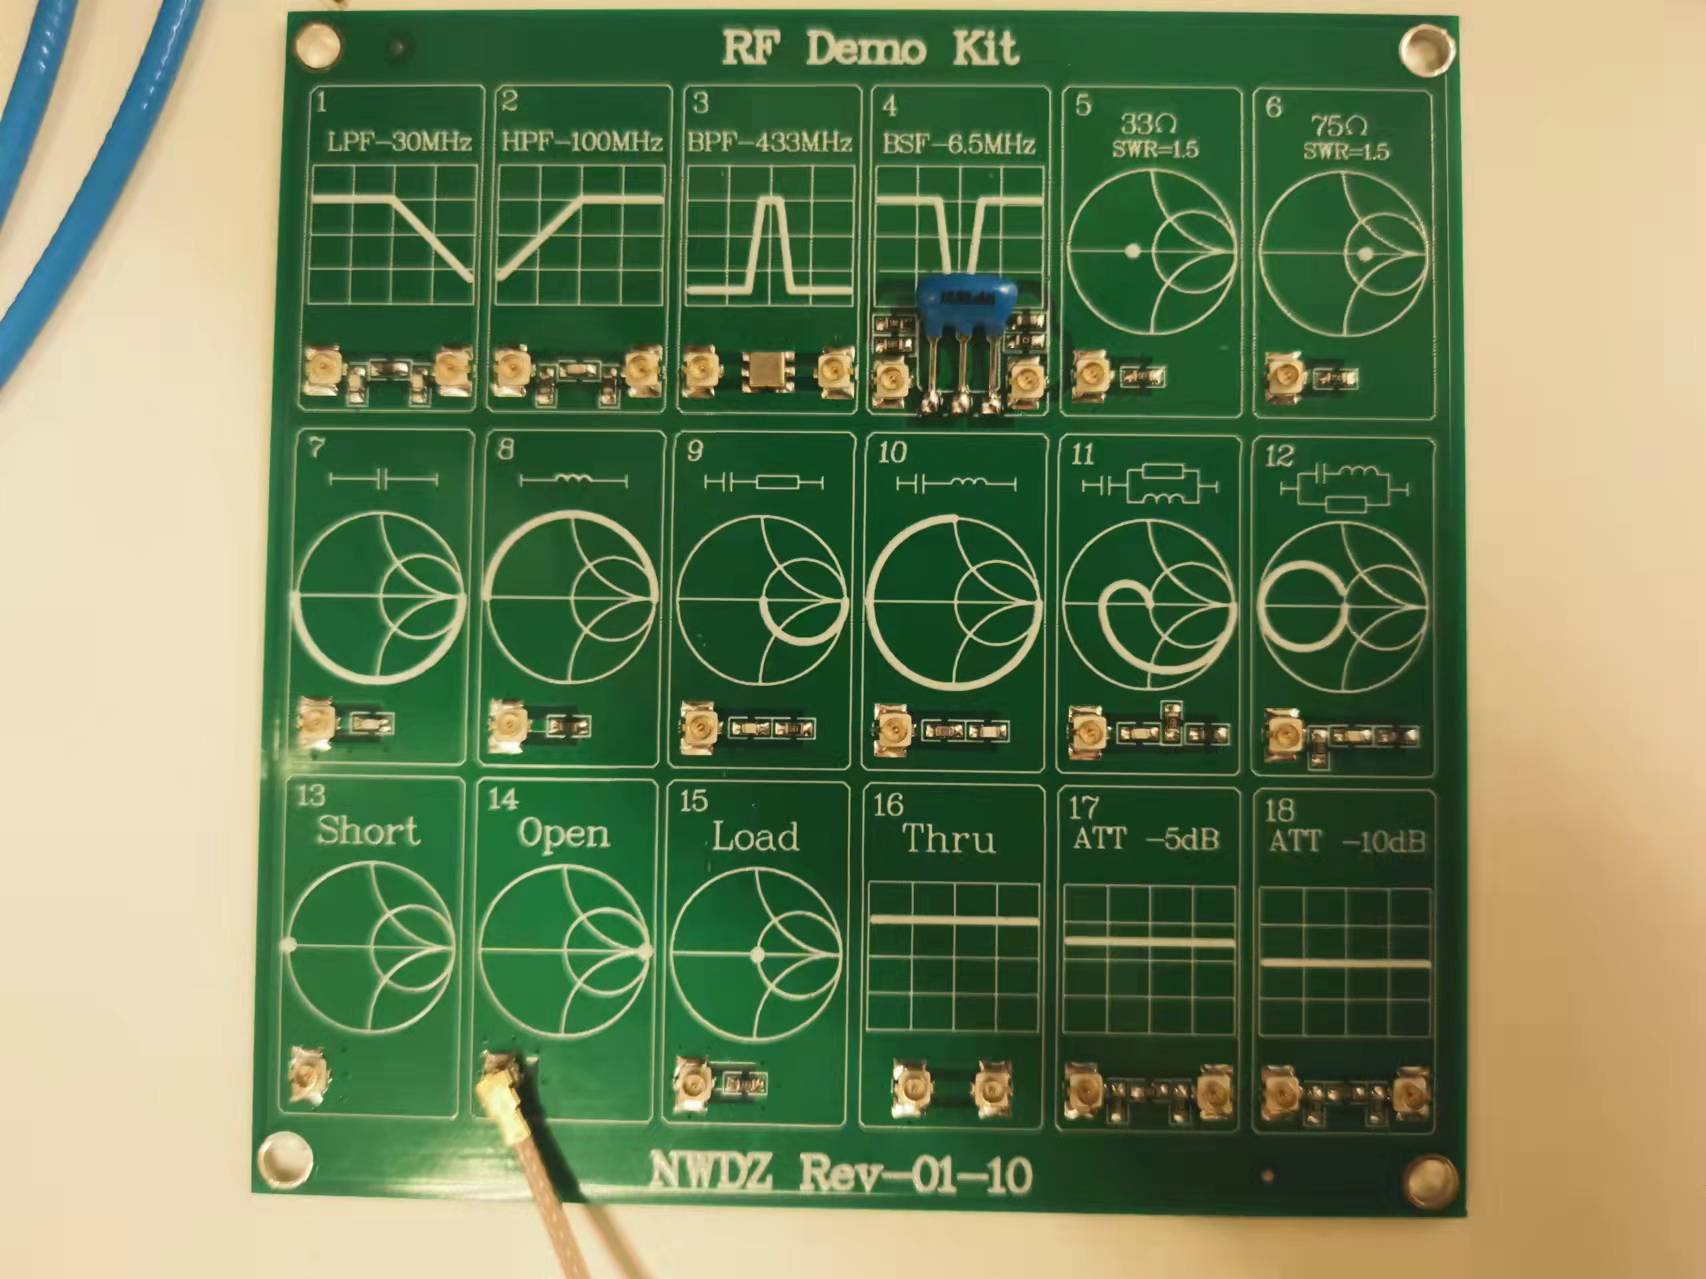
\includegraphics[width=.8\linewidth]{./pics/test_loads.jpg}
        \caption{Picture of RF Demo Kit NWDZ}
        \label{fig:test_loads}
    \end{subfigure}%
    \begin{subfigure}{.5\linewidth}
        \centering
        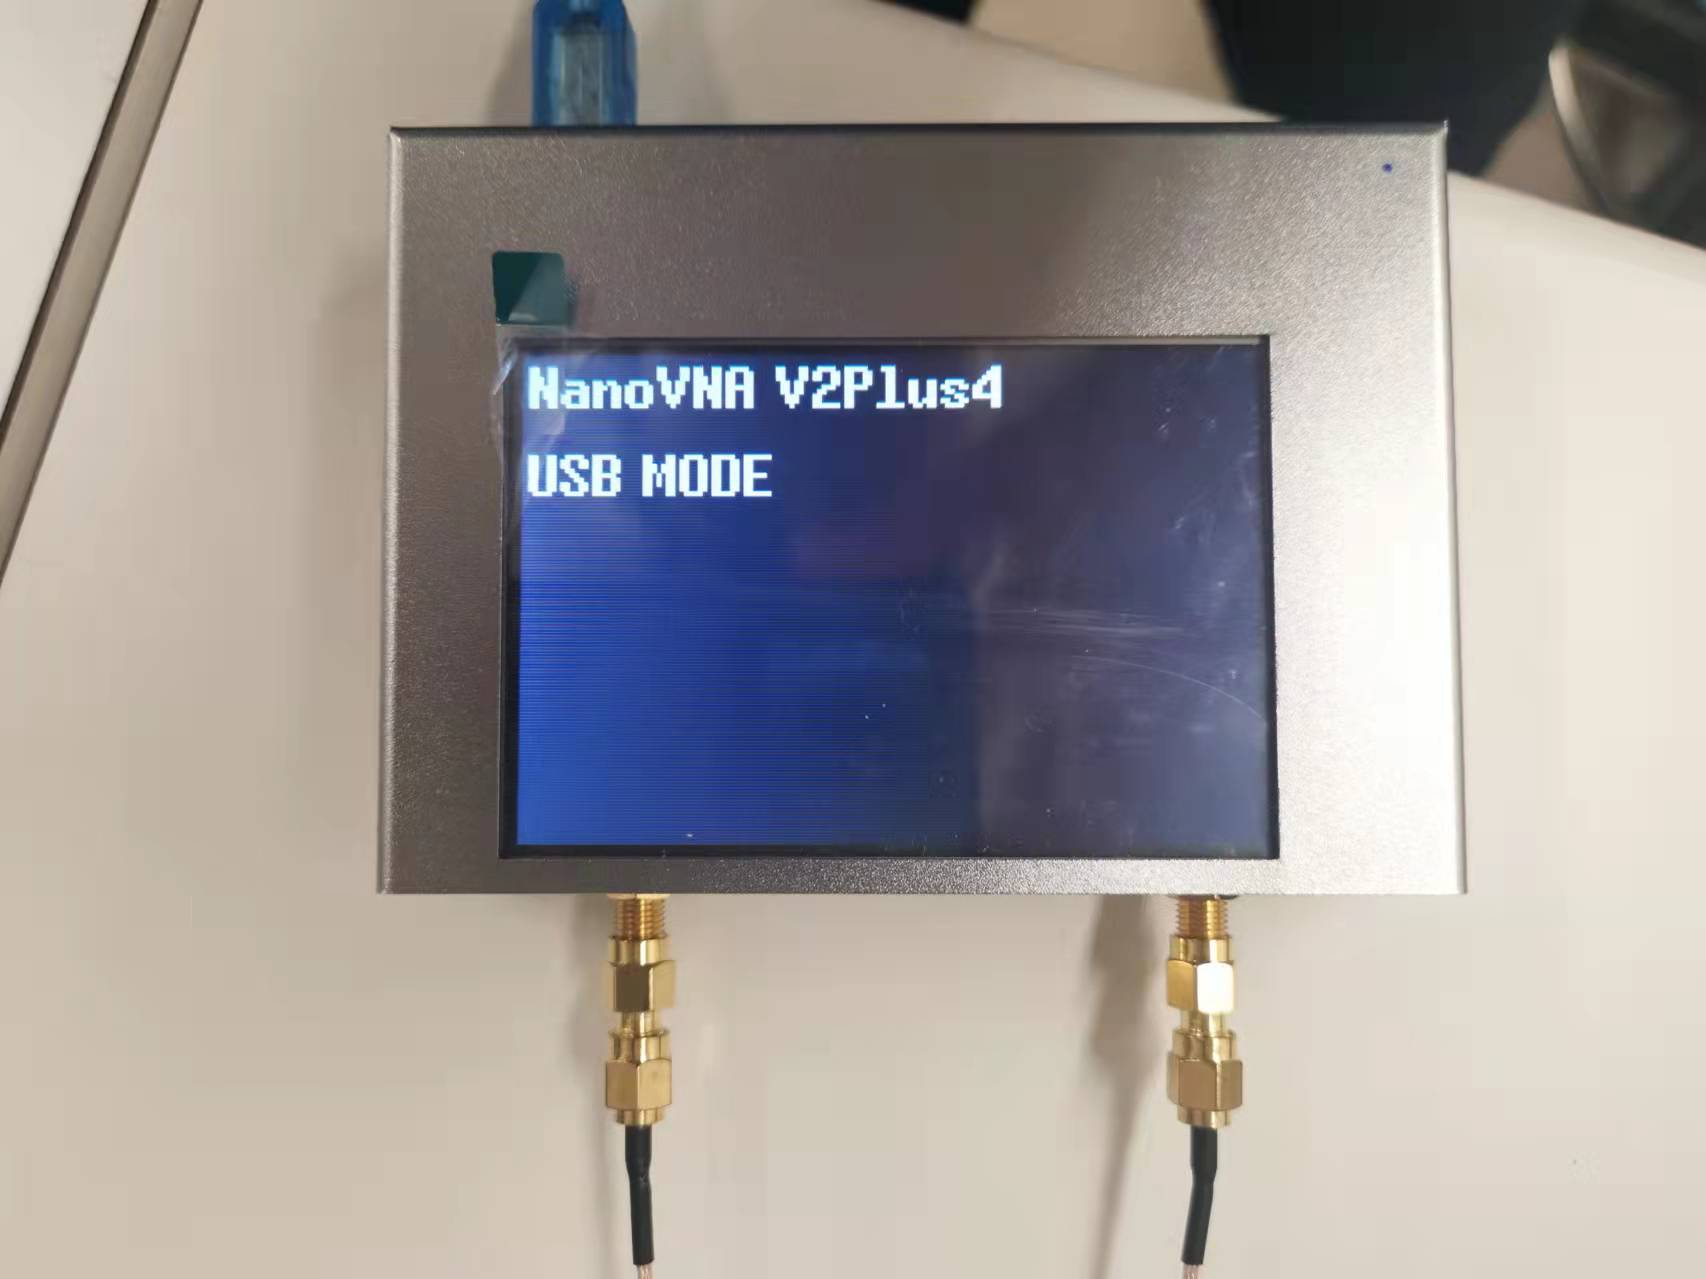
\includegraphics[width=.8\linewidth]{./pics/NanoVNA.jpg}
        \caption{Picture of NanoVNA}
        \label{fig:nanovna}
    \end{subfigure}
\end{figure}
Care is taken to calibrate the NanoVNA each time before use.

\section{Measurements and Results}

\subsection{Capacitor}

\subsection{Inductor}

\end{document}